\documentclass[8pt,a4paper]{extarticle}

\usepackage[T1]{fontenc}
\usepackage[utf8]{inputenc}
\usepackage{lmodern}
\usepackage[a4paper,margin=3mm,columnsep=2.5mm,footskip=2mm]{geometry}
\usepackage{multicol}
\usepackage{xcolor}
\usepackage{listings}
\usepackage{amsmath,amssymb}
\usepackage{array}
\usepackage{longtable}
\usepackage{booktabs}
\usepackage{enumitem}
\usepackage{titlesec}
\usepackage{tikz}
\usetikzlibrary{shapes.geometric,arrows.meta,positioning,calc,shapes.multipart,fit,backgrounds}
\usepackage[hidelinks]{hyperref}

% ---------- Kompakt-Layout ----------
\renewcommand{\normalsize}{\fontsize{5.85}{6.6}\selectfont}
\normalsize
\setlength{\parindent}{0pt}
\setlength{\parskip}{0.8pt}

% ---------- Farben ----------
\definecolor{loesungrahmen}{RGB}{20,90,50}
\definecolor{loesunghg}{RGB}{234,244,236}
\definecolor{codehg}{RGB}{246,246,246}
\definecolor{sqlkw}{RGB}{20,70,140}
\definecolor{sqlstr}{RGB}{150,30,30}
\definecolor{sqlcom}{RGB}{110,110,110}

\pagestyle{plain}
\newcommand{\Kopf}[1]{}

% ---------- kompakte \"Uberschriften ----------
\titleformat{\section}{\bfseries\fontsize{8}{9}\selectfont\color{loesungrahmen}}{}{0pt}{}
\titlespacing{\section}{0pt}{3pt}{1pt}
\titleformat{\subsection}{\bfseries\fontsize{7}{8}\selectfont}{}{0pt}{}
\titlespacing{\subsection}{0pt}{2pt}{0.5pt}
\titleformat{\subsubsection}{\bfseries\itshape\fontsize{5.85}{6.6}\selectfont}{}{0pt}{}
\titlespacing{\subsubsection}{0pt}{1.5pt}{0.5pt}

% ---------- L\"osungs-Umgebung (kompakt, ohne Box/Rahmen-Overhead) ----------
\newenvironment{loesung}[1][]{%
    \par\noindent{\bfseries\color{loesungrahmen}\small$\blacktriangleright$~L\"osung#1:}~%
}{\par\smallskip}

% ---------- SQL-Listings (kompakt) ----------
\lstdefinestyle{sqlstyle}{
    language=SQL,
    backgroundcolor=\color{codehg},
    basicstyle=\ttfamily\fontsize{5.15}{5.7}\selectfont,
    keywordstyle=\bfseries\color{sqlkw},
    stringstyle=\color{sqlstr},
    commentstyle=\itshape\color{sqlcom},
    showstringspaces=false,
    breaklines=true,
    breakatwhitespace=false,
    frame=none,
    aboveskip=1pt,
    belowskip=1pt,
    xleftmargin=1pt,
    numbers=none,
    tabsize=2,
    morekeywords={AUTO_INCREMENT,RLIKE,DELIMITER,ENGINE,IFNULL,NVL,STR\_TO\_DATE,DATE\_FORMAT,GROUP\_CONCAT,DATEDIFF},
}
\lstset{style=sqlstyle}

% ---------- ER-Diagramm Stile (Chen-Notation) ----------
\tikzset{
  entity/.style={rectangle, draw=black, thick, minimum width=2.3cm, minimum height=0.85cm, align=center, font=\bfseries\small, fill=blue!6},
  weakentity/.style={entity, double, double distance=1.5pt},
  rel/.style={diamond, draw=black, thick, aspect=1.6, align=center, font=\bfseries\tiny, fill=orange!12, inner sep=1pt, text width=1.7cm},
  attr/.style={ellipse, draw=black, minimum width=1.4cm, minimum height=0.55cm, align=center, font=\tiny, fill=white, inner sep=1pt},
  attrd/.style={attr, dashed},
  kante/.style={draw=black, thick},
  kardlabel/.style={font=\scriptsize\bfseries, fill=loesunghg, inner sep=1pt}
}
% Kardinalit\"atslabel an einem festen, kurzen Versatz vom Entit\"ats-/Beziehungsrand,
% unabh\"angig von der Linienf\"uhrung -- verhindert \"Uberlappungen mit der Raute.
\newcommand{\kard}[3]{\node[kardlabel] at ($(#1)!0.32!(#2)$) {#3};}

% ---------- Relationale-Modell Stile (Tabellenboxen) ----------
\tikzset{
  relbox/.style={rectangle split, rectangle split parts=2, draw=black, thick, rectangle split part align={center,left}, font=\ttfamily\scriptsize, fill=yellow!8, text width=3.9cm, inner sep=2pt},
}

\newcommand{\pk}[1]{\underline{#1}}
\newcommand{\relboxtitle}{\bfseries\sffamily\small}

\setlist[itemize]{topsep=1pt,itemsep=0pt,parsep=0pt,leftmargin=8pt}
\setlist[enumerate]{topsep=1pt,itemsep=0pt,parsep=0pt,leftmargin=8pt}

\begin{document}
{\centering\bfseries\fontsize{9}{10}\selectfont \"Ubung Anwendung von Datenbanksystemen -- Musterl\"osung (Kompaktversion)\par}
\begin{multicols}{4}

\section*{Aufgabe 1 \quad Entity Relationship Modell}
\Kopf{Aufgabe 1 Entity Relationship Modell}

\subsection*{1.2 \& 1.3 \quad Region/Land/Standort/Abteilung/Mitarbeiter}
Region(ID,Name) $\to$\,1:n\,$\to$ Land(ID,Name) $\to$\,1:n\,$\to$ Standort(ID,Stra\ss{}e,PLZ,Stadt,Bundesland) $\to$\,1:n\,$\to$ Abteilung(ID,Name) $\to$\,1:n\,$\to$ Mitarbeiter(ID,Vorname,Nachname,E-Mail,Telefonnummer,Einstelldatum,Gehalt,Provisionssatz). Mitarbeiter hat rekursive 1:n-Beziehung ``ist Vorgesetzter von'' auf sich selbst.

\begin{loesung}
Chen-Notation: Rechteck=Entit\"at, Raute=Beziehung, Ellipse=Attribut (unterstr.=Schl\"ussel, gestrichelt=abgeleitet), Zahlen=Kardinalit\"at.

\begin{center}
\resizebox{0.72\linewidth}{!}{%
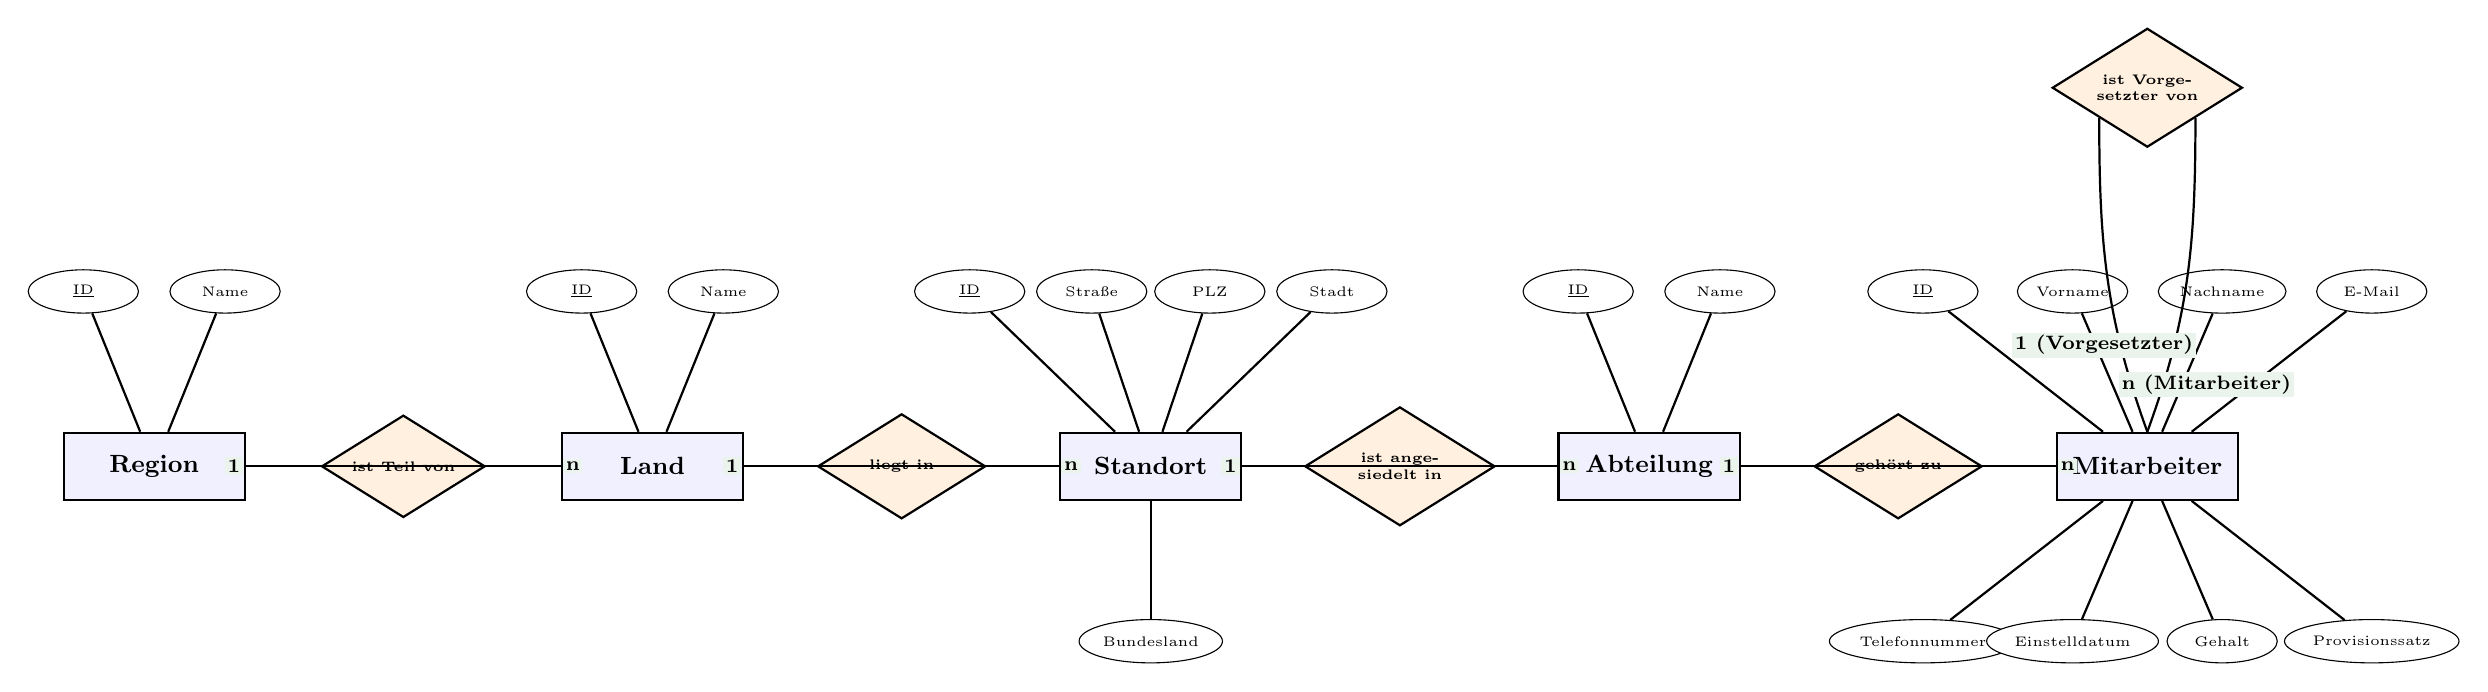
\begin{tikzpicture}[node distance=1.5cm and 4.0cm]

\node[entity] (region) {Region};
\node[attr, above=of region, xshift=-0.9cm] (r-id) {\pk{ID}};
\node[attr, above=of region, xshift=0.9cm] (r-name) {Name};
\draw[kante] (region) -- (r-id);
\draw[kante] (region) -- (r-name);

\node[entity, right=of region] (country) {Land};
\node[attr, above=of country, xshift=-0.9cm] (c-id) {\pk{ID}};
\node[attr, above=of country, xshift=0.9cm] (c-name) {Name};
\draw[kante] (country) -- (c-id);
\draw[kante] (country) -- (c-name);

\coordinate (mid1) at ($(region)!0.5!(country)$);
\node[rel] at (mid1) {ist Teil von};
\draw[kante] (region) -- (mid1);
\draw[kante] (mid1) -- (country);
\kard{region}{mid1}{1}
\kard{country}{mid1}{n}

\node[entity, right=of country] (location) {Standort};
\node[attr, above=of location, xshift=-2.3cm] (l-id) {\pk{ID}};
\node[attr, above=of location, xshift=-0.75cm] (l-str) {Stra\ss{}e};
\node[attr, above=of location, xshift=0.75cm] (l-plz) {PLZ};
\node[attr, above=of location, xshift=2.3cm] (l-stadt) {Stadt};
\node[attr, below=of location] (l-bl) {Bundesland};
\draw[kante] (location) -- (l-id);
\draw[kante] (location) -- (l-str);
\draw[kante] (location) -- (l-plz);
\draw[kante] (location) -- (l-stadt);
\draw[kante] (location) -- (l-bl);

\coordinate (mid2) at ($(country)!0.5!(location)$);
\node[rel] at (mid2) {liegt in};
\draw[kante] (country) -- (mid2);
\draw[kante] (mid2) -- (location);
\kard{country}{mid2}{1}
\kard{location}{mid2}{n}

\node[entity, right=of location] (dept) {Abteilung};
\node[attr, above=of dept, xshift=-0.9cm] (d-id) {\pk{ID}};
\node[attr, above=of dept, xshift=0.9cm] (d-name) {Name};
\draw[kante] (dept) -- (d-id);
\draw[kante] (dept) -- (d-name);

\coordinate (mid3) at ($(location)!0.5!(dept)$);
\node[rel] at (mid3) {ist ange-\\siedelt in};
\draw[kante] (location) -- (mid3);
\draw[kante] (mid3) -- (dept);
\kard{location}{mid3}{1}
\kard{dept}{mid3}{n}

\node[entity, right=of dept] (emp) {Mitarbeiter};
\node[attr, above=of emp, xshift=-2.85cm] (e-id) {\pk{ID}};
\node[attr, above=of emp, xshift=-0.95cm] (e-vor) {Vorname};
\node[attr, above=of emp, xshift=0.95cm] (e-nach) {Nachname};
\node[attr, above=of emp, xshift=2.85cm] (e-mail) {E-Mail};
\node[attr, below=of emp, xshift=-2.85cm] (e-tel) {Telefonnummer};
\node[attr, below=of emp, xshift=-0.95cm] (e-dat) {Einstelldatum};
\node[attr, below=of emp, xshift=0.95cm] (e-geh) {Gehalt};
\node[attr, below=of emp, xshift=2.85cm] (e-prov) {Provisionssatz};
\foreach \a in {e-id,e-vor,e-nach,e-mail,e-tel,e-dat,e-geh,e-prov}{\draw[kante] (emp) -- (\a);}

\coordinate (midE) at ($(dept)!0.5!(emp)$);
\node[rel] at (midE) {geh\"ort zu};
\draw[kante] (dept) -- (midE);
\draw[kante] (midE) -- (emp);
\kard{dept}{midE}{1}
\kard{emp}{midE}{n}

\node[rel, above=3.6cm of emp] (reportsto) {ist Vorge-\\setzter von};
\draw[kante] (emp.north) to[out=110,in=-90] (reportsto.south west);
\draw[kante] (reportsto.south east) to[out=-90,in=70] (emp.north);
\node[kardlabel] at ($(emp.north)+(-0.55,1.1)$) {1 (Vorgesetzter)};
\node[kardlabel] at ($(emp.north)+(0.75,0.6)$) {n (Mitarbeiter)};

\end{tikzpicture}}
\end{center}
\end{loesung}

\subsection*{1.4--1.6 \quad Projekte, Jobs, Besch\"aftigungsverlauf}
Projekt(ID,Name) steht in \textbf{n:m}-Beziehung ``arbeitet mit'' zu Mitarbeiter (Beziehungsattribute: Anteil, Projektleitung -- n:m-Beziehungen d\"urfen eigene Attribute tragen). Job(ID,Titel,Mindestgehalt*,Maximalgehalt* [*abgeleitet]) steht in 1:n-Beziehung ``ist angestellt als'' zu Mitarbeiter. Besch\"aftigungsverlauf (Start\_Datum,End\_Datum) ist eigener \emph{schwacher} Entit\"atstyp mit je einer 1:n-Beziehung zu Mitarbeiter/Abteilung/Job (da keine Paarkombination die Eintr\"age eindeutig identifiziert; PK sp\"ater: Mitarbeiter-ID+Start\_Datum).

\begin{loesung}
Vollst\"andiges ER-Modell (Basis f\"ur Aufgabe 2). Attribute von Region/Land/Standort/Abteilung/Mitarbeiter siehe Diagramm oben.

\begin{center}
\resizebox{0.72\linewidth}{!}{%
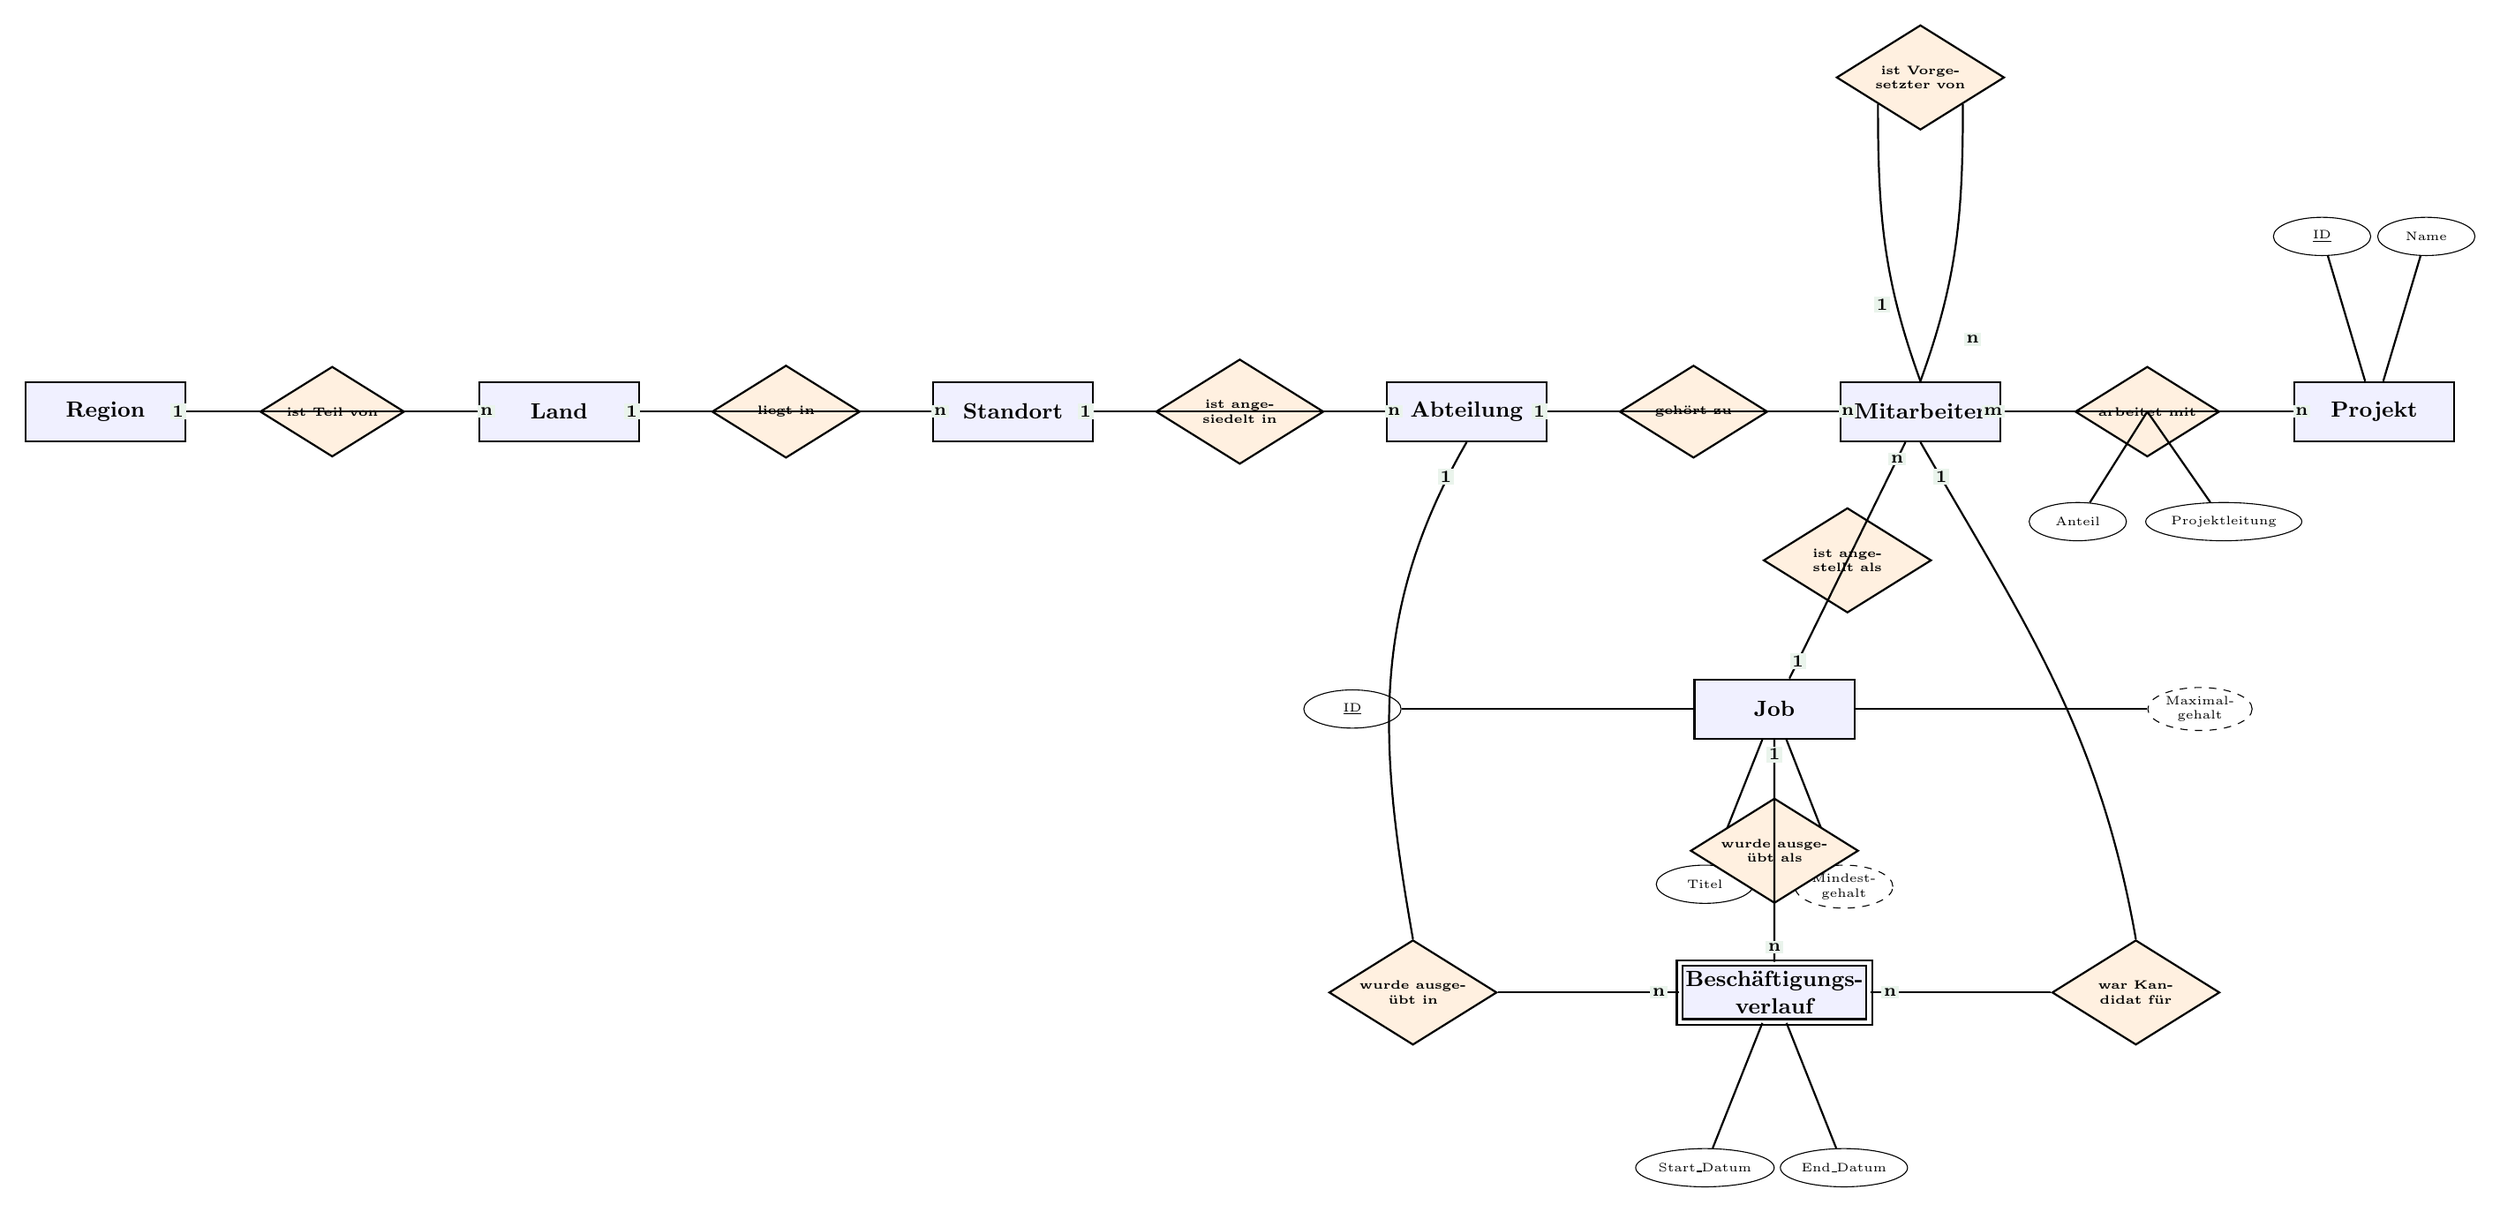
\begin{tikzpicture}[node distance=1.8cm and 4.2cm]

\node[entity] (region) {Region};
\node[entity, right=of region] (country) {Land};
\node[entity, right=of country] (location) {Standort};
\node[entity, right=of location] (dept) {Abteilung};
\node[entity, right=of dept] (emp) {Mitarbeiter};
\node[entity, right=of emp] (proj) {Projekt};
\node[attr, above=of proj, xshift=-0.75cm] (p-id) {\pk{ID}};
\node[attr, above=of proj, xshift=0.75cm] (p-name) {Name};
\draw[kante] (proj) -- (p-id);
\draw[kante] (proj) -- (p-name);

\coordinate (m1) at ($(region)!0.5!(country)$); \node[rel] at (m1) {ist Teil von};
\draw[kante] (region) -- (m1); \draw[kante] (m1) -- (country);
\kard{region}{m1}{1} \kard{country}{m1}{n}

\coordinate (m2) at ($(country)!0.5!(location)$); \node[rel] at (m2) {liegt in};
\draw[kante] (country) -- (m2); \draw[kante] (m2) -- (location);
\kard{country}{m2}{1} \kard{location}{m2}{n}

\coordinate (m3) at ($(location)!0.5!(dept)$); \node[rel] at (m3) {ist ange-\\siedelt in};
\draw[kante] (location) -- (m3); \draw[kante] (m3) -- (dept);
\kard{location}{m3}{1} \kard{dept}{m3}{n}

\coordinate (m4) at ($(dept)!0.5!(emp)$); \node[rel] at (m4) {geh\"ort zu};
\draw[kante] (dept) -- (m4); \draw[kante] (m4) -- (emp);
\kard{dept}{m4}{1} \kard{emp}{m4}{n}

\node[rel, above=3.6cm of emp] (reportsto) {ist Vorge-\\setzter von};
\draw[kante] (emp.north) to[out=110,in=-90] (reportsto.south west);
\draw[kante] (reportsto.south east) to[out=-90,in=70] (emp.north);
\node[kardlabel] at ($(emp.north)+(-0.55,1.1)$) {1};
\node[kardlabel] at ($(emp.north)+(0.75,0.6)$) {n};

\coordinate (m5) at ($(emp)!0.5!(proj)$); \node[rel] at (m5) {arbeitet mit};
\draw[kante] (emp) -- (m5); \draw[kante] (m5) -- (proj);
\kard{emp}{m5}{m} \kard{proj}{m5}{n}
\node[attr, below=1.3cm of m5, xshift=-1.0cm] (rp-anteil) {Anteil};
\node[attr, below=1.3cm of m5, xshift=1.1cm] (rp-lead) {Projektleitung};
\draw[kante] (m5) -- (rp-anteil);
\draw[kante] (m5) -- (rp-lead);

\node[entity, below right=3.4cm and 2.1cm of dept] (job) {Job};
\node[attr, left=of job] (j-id) {\pk{ID}};
\node[attr, below=of job, xshift=-1.0cm] (j-titel) {Titel};
\node[attrd, below=of job, xshift=1.0cm] (j-min) {Mindest-\\gehalt};
\node[attrd, right=of job] (j-max) {Maximal-\\gehalt};
\draw[kante] (job) -- (j-id);
\draw[kante] (job) -- (j-titel);
\draw[kante] (job) -- (j-min);
\draw[kante] (job) -- (j-max);
\coordinate (m6) at ($(job)!0.5!(emp)$); \node[rel] at (m6) {ist ange-\\stellt als};
\draw[kante] (job) -- (m6); \draw[kante] (m6) -- (emp);
\kard{job}{m6}{1} \kard{emp}{m6}{n}

\node[weakentity, below=3.2cm of job] (jh) {Besch\"aftigungs-\\verlauf};
\node[attr, below=of jh, xshift=-1.0cm] (jh-start) {Start\_Datum};
\node[attr, below=of jh, xshift=1.0cm] (jh-end) {End\_Datum};
\draw[kante] (jh) -- (jh-start);
\draw[kante] (jh) -- (jh-end);

\coordinate (m7) at ($(job)!0.5!(jh)$); \node[rel] at (m7) {wurde ausge-\\\"ubt als};
\draw[kante] (job) -- (m7); \draw[kante] (m7) -- (jh);
\kard{job}{m7}{1} \kard{jh}{m7}{n}

\node[rel, left=2.6cm of jh] (workedhere) {wurde ausge-\\\"ubt in};
\draw[kante] (workedhere) -- (jh);
\kard{jh}{workedhere}{n}
\draw[kante] (dept.south) to[out=-120,in=100] (workedhere.north);
\node[kardlabel] at ($(dept.south)+(-0.3,-0.5)$) {1};

\node[rel, right=2.6cm of jh] (wascand) {war Kandidat f\"ur};
\draw[kante] (jh) -- (wascand);
\kard{jh}{wascand}{n}
\draw[kante] (emp.south) to[out=-60,in=100] (wascand.north);
\node[kardlabel] at ($(emp.south)+(0.3,-0.5)$) {1};

\end{tikzpicture}}
\end{center}
\end{loesung}


\section*{Aufgabe 2 \quad relationales Modell}
\Kopf{Aufgabe 2 relationales Modell}

Im Rahmen dieser \"Ubung soll aus dem Entity-Relationship-Modell (siehe L\"osung zu Aufgabe 1.6) ein relationales Modell erstellt werden.

\subsection*{2.1 \quad Relationen der Entit\"atstypen}
\"Uberf\"uhren Sie alle Entit\"atstypen aus dem Entity-Relationship-Modell in das relationale Modell.

\begin{loesung}
Jeder Entit\"atstyp wird zun\"achst 1:1 in eine Relation \"uberf\"uhrt; die Schl\"usselattribute des Entit\"atstyps werden zum Prim\"arschl\"ussel der Relation:
\begin{itemize}
\item \texttt{region(\pk{region\_id}, region\_name)}
\item \texttt{country(\pk{country\_id}, country\_name)}
\item \texttt{location(\pk{location\_id}, street\_address, postal\_code, city, state\_province)}
\item \texttt{department(\pk{department\_id}, department\_name)}
\item \texttt{employee(\pk{employee\_id}, first\_name, last\_name, email, phone\_number, hire\_date, salary, commission\_pct)}
\item \texttt{job(\pk{job\_id}, job\_title, min\_salary, max\_salary)}
\item \texttt{project(\pk{project\_id}, project\_name)}
\end{itemize}
Die abgeleiteten Attribute \texttt{min\_salary}/\texttt{max\_salary} werden trotz ihrer Ableitbarkeit als gew\"ohnliche (materialisierte) Spalten gef\"uhrt, da SQL keine automatisch berechneten, immer aktuellen Attribute ohne Trigger/View kennt.
\end{loesung}

\subsection*{2.2 \quad Relationen der Beziehungstypen}
\"Uberf\"uhren Sie alle Beziehungstypen des Entity-Relationship-Modells in das relationale Modell. Achten Sie insbesondere auf die korrekte Definition der Prim\"arschl\"ussel.

\begin{loesung}
Grundregel: 1:n-Beziehungen ben\"otigen \emph{keine} eigene Relation -- der Fremdschl\"ussel wird stattdessen als zus\"atzliche Spalte in die Relation auf der ``n''-Seite aufgenommen. Nur n:m-Beziehungen (und mehrstellige/assoziative Beziehungen) ben\"otigen eine eigene Verbindungsrelation.

\begin{itemize}
\item \emph{ist Teil von} (1:n): \texttt{country.region\_id} $\to$ \texttt{region.region\_id}
\item \emph{liegt in} (1:n): \texttt{location.country\_id} $\to$ \texttt{country.country\_id}
\item \emph{ist angesiedelt in} (1:n): \texttt{department.location\_id} $\to$ \texttt{location.location\_id}
\item \emph{geh\"ort zu} (1:n): \texttt{employee.department\_id} $\to$ \texttt{department.department\_id}
\item \emph{ist angestellt als} (1:n): \texttt{employee.job\_id} $\to$ \texttt{job.job\_id}
\item \emph{ist Vorgesetzter von} (1:n, rekursiv): \texttt{employee.manager\_id} $\to$ \texttt{employee.employee\_id}
\item \emph{arbeitet mit} (\textbf{n:m} $\Rightarrow$ eigene Relation): \\
\texttt{employee2project(\pk{employee\_id}, \pk{project\_id}, assoc\_pct, is\_project\_lead)} \\
mit \texttt{employee\_id} $\to$ \texttt{employee.employee\_id} und \texttt{project\_id} $\to$ \texttt{project.project\_id}. Der Prim\"arschl\"ussel besteht aus \emph{beiden} Fremdschl\"usseln, da genau diese Kombination die Beziehung eindeutig identifiziert.
\item \emph{Besch\"aftigungsverlauf} (drei 1:n-Beziehungen zu einem assoziativen Entit\"atstyp $\Rightarrow$ eigene Relation): \\
\texttt{job\_history(\pk{employee\_id}, \pk{start\_date}, end\_date, job\_id, department\_id)} \\
mit \texttt{employee\_id} $\to$ \texttt{employee.employee\_id}, \texttt{job\_id} $\to$ \texttt{job.job\_id}, \texttt{department\_id} $\to$ \texttt{department.department\_id}. Als Prim\"arschl\"ussel wird -- wie in der Aufgabenstellung vorgegeben -- \texttt{(employee\_id, start\_date)} verwendet (ein Mitarbeiter kann zu einem gegebenen Startdatum immer nur einen Besch\"aftigungsabschnitt beginnen).
\end{itemize}
\end{loesung}

\subsection*{2.3 \quad Vereinfachung des relationalen Modells}
Vereinfachen Sie das entstandene relationale Modell durch geeignete Zusammenfassung der Relationen.

\begin{loesung}
Da s\"amtliche 1:n-Beziehungen bereits in Schritt 2.2 direkt als Fremdschl\"ussel-Spalte in die referenzierende Relation integriert wurden (statt eigene Beziehungsrelationen anzulegen), ist keine weitere Zusammenfassung mehr n\"otig oder m\"oglich: Eine zus\"atzliche Verschmelzung w\"are nur bei 1:1-Beziehungen sinnvoll (hier nicht vorhanden) oder wenn f\"alschlicherweise auch f\"ur 1:n-Beziehungen eigene Relationen angelegt worden w\"aren. Das vereinfachte relationale Modell besteht somit aus genau 9 Relationen: \texttt{region, country, location, department, job, employee, project, employee2project, job\_history}.
\end{loesung}

\subsection*{2.4 \quad Datentypen}
Erweitern Sie die Relationen des vereinfachten relationalen Modells um passende Datentypen.

\begin{loesung}
Die folgende Abbildung zeigt das vollst\"andige relationale Modell (= HR-Schema) inklusive Datentypen, Prim\"ar- (unterstrichen) und Fremdschl\"usseln (Pfeile). Es ist identisch mit dem in Aufgabe 3.6/4 vorausgesetzten Schema und bildet die Grundlage f\"ur alle folgenden \"Ubungen.

\begin{center}
\resizebox{0.85\linewidth}{!}{%
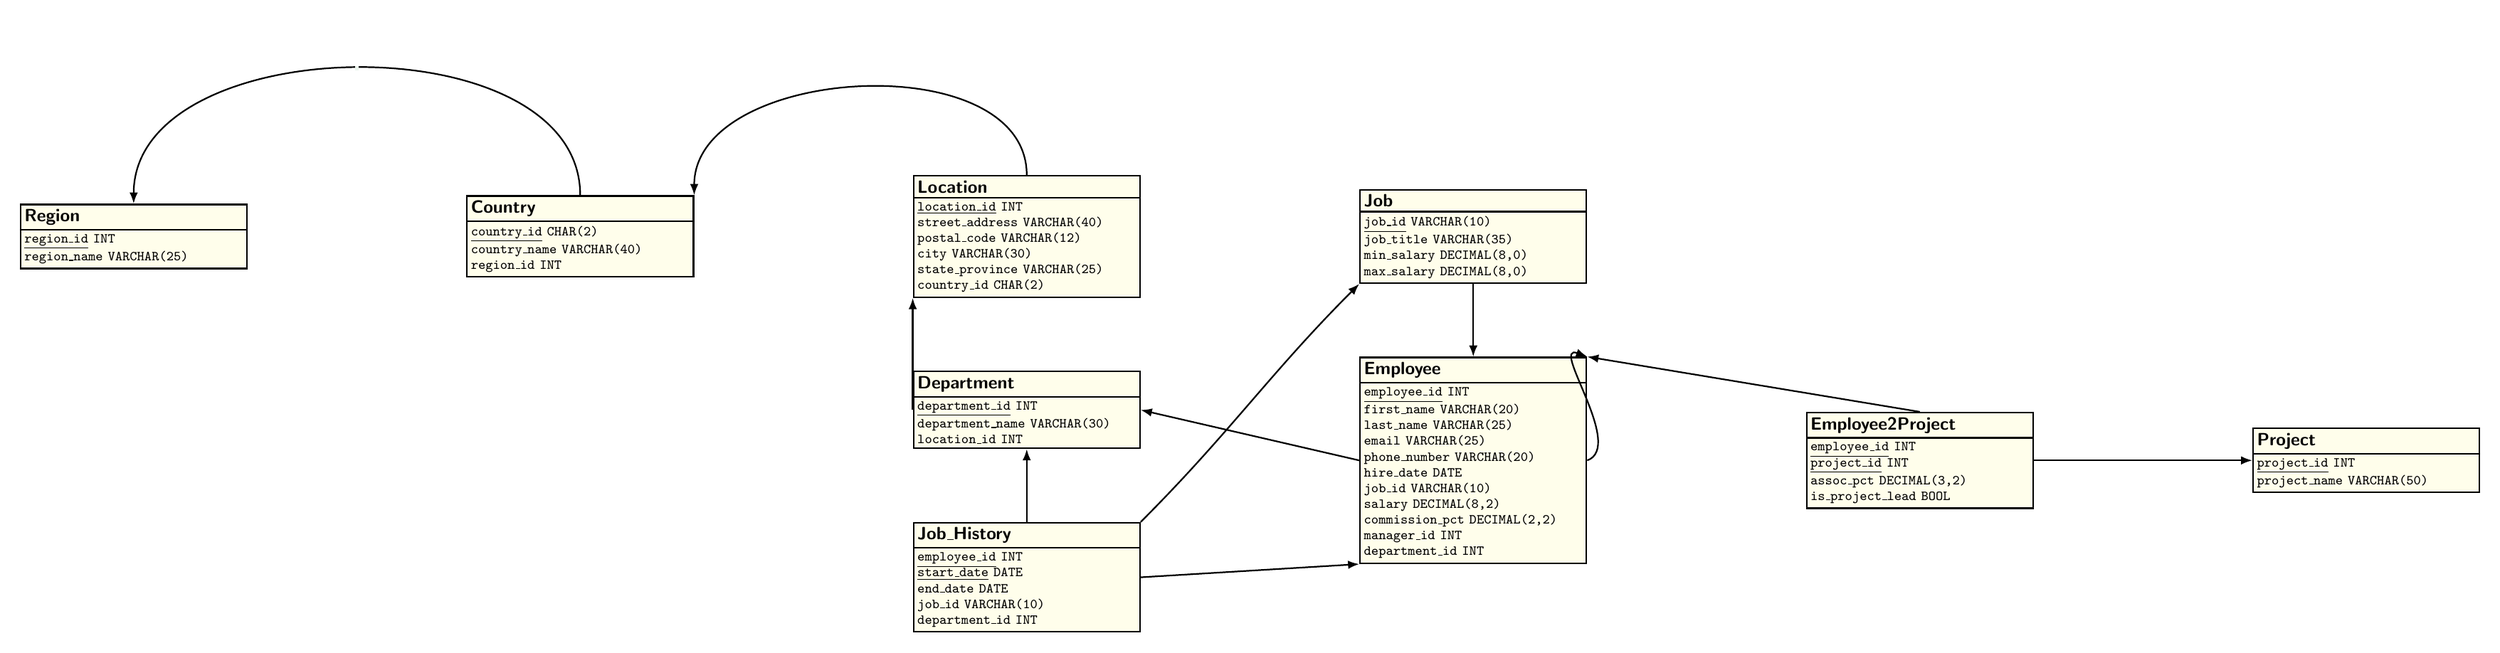
\begin{tikzpicture}[node distance=1.3cm and 1.6cm]

\node[relbox] (region) {\relboxtitle Region
\nodepart{two} \pk{region\_id} INT\\ region\_name VARCHAR(25)};

\node[relbox, right=3.9cm of region] (country) {\relboxtitle Country
\nodepart{two} \pk{country\_id} CHAR(2)\\ country\_name VARCHAR(40)\\ region\_id INT};

\node[relbox, right=3.9cm of country] (location) {\relboxtitle Location
\nodepart{two} \pk{location\_id} INT\\ street\_address VARCHAR(40)\\ postal\_code VARCHAR(12)\\ city VARCHAR(30)\\ state\_province VARCHAR(25)\\ country\_id CHAR(2)};

\node[relbox, below=of location] (department) {\relboxtitle Department
\nodepart{two} \pk{department\_id} INT\\ department\_name VARCHAR(30)\\ location\_id INT};

\node[relbox, right=3.9cm of location] (job) {\relboxtitle Job
\nodepart{two} \pk{job\_id} VARCHAR(10)\\ job\_title VARCHAR(35)\\ min\_salary DECIMAL(8,0)\\ max\_salary DECIMAL(8,0)};

\node[relbox, below=of job] (employee) {\relboxtitle Employee
\nodepart{two} \pk{employee\_id} INT\\ first\_name VARCHAR(20)\\ last\_name VARCHAR(25)\\ email VARCHAR(25)\\ phone\_number VARCHAR(20)\\ hire\_date DATE\\ job\_id VARCHAR(10)\\ salary DECIMAL(8,2)\\ commission\_pct DECIMAL(2,2)\\ manager\_id INT\\ department\_id INT};

\node[relbox, below=of department] (jobhist) {\relboxtitle Job\_History
\nodepart{two} \pk{employee\_id} INT\\ \pk{start\_date} DATE\\ end\_date DATE\\ job\_id VARCHAR(10)\\ department\_id INT};

\node[relbox, right=3.9cm of employee] (e2p) {\relboxtitle Employee2Project
\nodepart{two} \pk{employee\_id} INT\\ \pk{project\_id} INT\\ assoc\_pct DECIMAL(3,2)\\ is\_project\_lead BOOL};

\node[relbox, right=3.9cm of e2p] (project) {\relboxtitle Project
\nodepart{two} \pk{project\_id} INT\\ project\_name VARCHAR(50)};

\draw[-{Latex[length=2mm]}, thick] (country.north) to[out=90,in=90] node[kardlabel,midway]{} (region.north);
\draw[-{Latex[length=2mm]}, thick] (location.north) to[out=90,in=90] (country.north east);
\draw[-{Latex[length=2mm]}, thick] (department.west) -- (location.south west);
\draw[-{Latex[length=2mm]}, thick] (job.south) -- (employee.north);
\draw[-{Latex[length=2mm]}, thick] (employee.west) -- (department.east);
\draw[-{Latex[length=2mm]}, thick] (jobhist.north) -- (department.south);
\draw[-{Latex[length=2mm]}, thick] (jobhist.east) -- (employee.south west);
\draw[-{Latex[length=2mm]}, thick] (jobhist.north east) to[out=45,in=-135] (job.south west);
\draw[-{Latex[length=2mm]}, thick] (e2p.north) -- (employee.north east);
\draw[-{Latex[length=2mm]}, thick] (e2p.east) -- (project.west);
\draw[-{Latex[length=2mm]}, thick] (employee.east) to[out=20,in=160] (employee.east |- employee.north);

\end{tikzpicture}}
\end{center}
\textit{Legende:} Pfeile zeigen jeweils vom Fremdschl\"ussel auf den referenzierten Prim\"arschl\"ussel. Der Selbstbezug \texttt{employee.manager\_id} $\to$ \texttt{employee.employee\_id} ist als kleine Schleife an der \emph{Employee}-Box angedeutet. Die vollst\"andigen \texttt{CREATE TABLE}-Anweisungen inkl.\ aller Fremdschl\"ussel folgen in der L\"osung zu Aufgabe 4.
\end{loesung}


\section*{Aufgabe 3 \quad Normalisierung}
\Kopf{Aufgabe 3 Normalisierung}

\subsection*{3.1 \quad Normalformen}
Gegeben sei das folgende relationale Modell zur Verwaltung der offenen Rechnungen eines Onlineshops inkl.\ Beispieldaten:

\begin{center}
\small
\begin{tabular}{cccccc c}
\toprule
\pk{RNr} & KDNr & Name & Wohnort & Pos & Datum & Betrag\\
\midrule
1 & 1 & M\"uller & M\"unchen & 3 & 01.11.2021 & 60\\
2 & 1 & M\"uller & M\"unchen & 2 & 23.05.2021 & 90\\
3 & 2 & Huber & N\"urnberg & 2 & 09.03.2022 & 90\\
4 & 2 & Huber & N\"urnberg & 2 & 14.02.2022 & 70\\
5 & 3 & Meier & Augsburg & 3 & 20.06.2022 & 110\\
6 & 4 & Meier & M\"unchen & 4 & 07.04.2022 & 90\\
\bottomrule
\end{tabular}
\end{center}

\subsubsection*{3.1.1 \quad 2. Normalform}
Warum k\"onnen nur Relationen mit zusammengesetzten Schl\"usseln die 2.\,NF verletzen?
\begin{loesung}
2.\,NF verletzt = ein Nicht-Schl\"usselattribut h\"angt nur von einer \emph{echten Teilmenge} des Schl\"ussels ab (partielle Abh\"angigkeit). Ein einwertiger Schl\"ussel hat keine nichttriviale echte Teilmenge $\Rightarrow$ partielle Abh\"angigkeit strukturell unm\"oglich. Erst bei zusammengesetztem Schl\"ussel kann ein Attribut von einem Teil davon abh\"angen.
\end{loesung}

\subsection*{3.2 \quad Funktionale Abh\"angigkeiten}
\begin{loesung}
Schl\"ussel: \texttt{RNr}. FDs: RNr$\to$KDNr,Pos,Datum,Betrag; KDNr$\to$Name,Wohnort. Transitiv: RNr$\to$Name,Wohnort.
\end{loesung}

\subsection*{3.3 \quad 3. Normalform}
\begin{loesung}
\textbf{Versto\ss{}:} Name/Wohnort h\"angen nur transitiv via KDNr vom Schl\"ussel RNr ab. \textbf{Anomalien:} \"Anderung (Umzug $\Rightarrow$ mehrere Zeilen \"andern), Einf\"ugen (Kunde ohne Rechnung nicht speicherbar), L\"oschen (letzte Rechnung l\"oschen $\Rightarrow$ Kundendaten weg). \textbf{3.\,NF:} \texttt{Kunde(\pk{KDNr},Name,Wohnort)}, \texttt{Rechnung(\pk{RNr},KDNr,Pos,Datum,Betrag)} mit KDNr$\to$Kunde.KDNr.
\end{loesung}

\subsection*{3.4 \quad Boyce-Codd Normalform}
\begin{loesung}
Beide Relationen: einziger Determinant ist jeweils der (einwertige) Schl\"ussel selbst $\Rightarrow$ \textbf{Zerlegung aus 3.3 ist bereits BCNF}, keine weitere n\"otig.
\end{loesung}

\subsection*{3.5 \quad Normalform Hochschul-Schema}
\begin{loesung}
Dozent/Studierende/Vorlesung: einwertiger Schl\"ussel $\Rightarrow$ BCNF. Kapitel(\pk{Modulnr},\pk{\"Uberschrift},Inhalt): Inhalt h\"angt von beiden Teilen ab $\Rightarrow$ BCNF. h\"ort: nur Schl\"usselattribute $\Rightarrow$ trivial BCNF. Raumbelegung(\pk{Raum},\pk{Tag},\pk{Zeit},\pk{Semester},Modulnr): Modulnr h\"angt vom vollst\"andigen Schl\"ussel ab $\Rightarrow$ BCNF. Pr\"ufung: einwertig $\Rightarrow$ BCNF. schreibt(\pk{Modulnr},\pk{Pr\"ufungsID},\pk{Matrikelnr},Note): Note h\"angt von voller Kombination ab $\Rightarrow$ BCNF. \textbf{Ergebnis: gesamtes Schema in BCNF.}
\end{loesung}

\subsection*{3.6 \quad Normalform HR-Schema}
\begin{loesung}
Alle 9 Relationen: einwertiger PK oder zusammengesetzter PK mit voller Abh\"angigkeit (\texttt{job\_history}: Job/Abteilung h\"angen von Mitarbeiter+Startdatum; \texttt{employee2project}: assoc\_pct/is\_project\_lead h\"angen von Mitarbeiter+Projekt) $\Rightarrow$ \textbf{BCNF}. Sonderf\"alle: (1) \texttt{postal\_code}$\to$\texttt{city} w\"are transitiv/3NF-Versto\ss{}, gilt hier aber nicht global (NULL-PLZ bei London/Rom etc.) $\Rightarrow$ kein Versto\ss{}. (2) \texttt{job.min/max\_salary} sind aus \texttt{employee.salary} abgeleitet -- kein BCNF-Versto\ss{} \emph{innerhalb} \texttt{job}, aber relationen\"ubergreifende Redundanz (manuell konsistent zu halten).
\end{loesung}


\section*{Aufgabe 4 \quad SQL Data Definition Language -- Teil 1}
\Kopf{Aufgabe 4 SQL Data Definition Language - Teil 1}

Ziel: Im Rahmen dieser \"Ubung sollen die grundlegenden SQL-Befehle f\"ur die Implementierung des HR-Schemas mit Hilfe eines MariaDB-DBS erstellt werden.

\subsection*{4.2 \quad Schema-Erstellung}
Neues Schema ``hr'' erstellen (Datei \texttt{HR\_setupDB.sql}, beliebig oft ausf\"uhrbar).

\begin{loesung}
\begin{lstlisting}
DROP DATABASE IF EXISTS hr;
CREATE DATABASE hr;
USE hr;
\end{lstlisting}
Das \texttt{DROP DATABASE IF EXISTS} stellt sicher, dass das Skript beliebig oft ausgef\"uhrt werden kann und das Schema bei jedem Lauf komplett neu aufgebaut wird.
\end{loesung}

\subsection*{4.3 \quad Relationen, Attribute und Datentypen}
Alle Relationen mit Attributen/Datentypen/PK im ``hr''-Schema erstellen.

\begin{loesung}
\begin{lstlisting}
CREATE TABLE region (
    region_id   INT NOT NULL,
    region_name VARCHAR(25),
    PRIMARY KEY (region_id)
);

CREATE TABLE country (
    country_id   CHAR(2) NOT NULL,
    country_name VARCHAR(40),
    region_id    INT NOT NULL,
    PRIMARY KEY (country_id)
);

CREATE TABLE location (
    location_id    INT NOT NULL AUTO_INCREMENT,
    street_address VARCHAR(40),
    postal_code    VARCHAR(12),
    city           VARCHAR(30) NOT NULL,
    state_province VARCHAR(25),
    country_id     CHAR(2) NOT NULL,
    PRIMARY KEY (location_id)
);

CREATE TABLE department (
    department_id   INT NOT NULL,
    department_name VARCHAR(30) NOT NULL,
    location_id     INT,
    PRIMARY KEY (department_id)
);

CREATE TABLE job (
    job_id     VARCHAR(10) NOT NULL,
    job_title  VARCHAR(35) NOT NULL,
    min_salary DECIMAL(8,0),
    max_salary DECIMAL(8,0),
    PRIMARY KEY (job_id)
);

CREATE TABLE employee (
    employee_id    INT NOT NULL,
    first_name     VARCHAR(20),
    last_name      VARCHAR(25) NOT NULL,
    email          VARCHAR(25) NOT NULL,
    phone_number   VARCHAR(20),
    hire_date      DATE NOT NULL,
    job_id         VARCHAR(10) NOT NULL,
    salary         DECIMAL(8,2) NOT NULL,
    commission_pct DECIMAL(2,2),
    manager_id     INT,
    department_id  INT,
    PRIMARY KEY (employee_id)
);

CREATE TABLE job_history (
    employee_id   INT NOT NULL,
    start_date    DATE NOT NULL,
    end_date      DATE NOT NULL,
    job_id        VARCHAR(10) NOT NULL,
    department_id INT NOT NULL,
    PRIMARY KEY (employee_id, start_date)
);

CREATE TABLE project (
    project_id   INT NOT NULL,
    project_name VARCHAR(50),
    PRIMARY KEY (project_id)
);

CREATE TABLE employee2project (
    employee_id     INT NOT NULL,
    project_id      INT NOT NULL,
    assoc_pct       DECIMAL(3,2),
    is_project_lead BOOL,
    PRIMARY KEY (employee_id, project_id)
);
\end{lstlisting}
\emph{Optionalit\"at der Attribute:} Attribute, die laut Aufgabenstellung immer vorhanden sein m\"ussen (z.\,B.\ Namen, Datumswerte, E-Mail), sind \texttt{NOT NULL}; optionale Attribute (z.\,B.\ \texttt{commission\_pct}, \texttt{manager\_id} beim CEO, \texttt{department\_id} vor Zuordnung) bleiben nullable.
\end{loesung}

\subsection*{4.4 \quad Fremdschl\"usselbeziehungen}
\subsubsection*{4.4.1 \quad Implementierung}
Erg\"anzen Sie die notwendigen SQL-Befehle, um die Fremdschl\"usselbeziehungen zwischen den Relationen unter Ber\"ucksichtigung der vorgegebenen Referenzierungsoptionen herzustellen.

\begin{loesung}
\begin{lstlisting}
ALTER TABLE country
    ADD FOREIGN KEY (region_id) REFERENCES region(region_id)
        ON UPDATE CASCADE ON DELETE RESTRICT;

ALTER TABLE location
    ADD FOREIGN KEY (country_id) REFERENCES country(country_id)
        ON UPDATE CASCADE ON DELETE RESTRICT;

ALTER TABLE department
    ADD FOREIGN KEY (location_id) REFERENCES location(location_id)
        ON UPDATE CASCADE ON DELETE RESTRICT;

ALTER TABLE employee
    ADD FOREIGN KEY (job_id) REFERENCES job(job_id)
        ON UPDATE CASCADE ON DELETE RESTRICT,
    ADD FOREIGN KEY (department_id) REFERENCES department(department_id)
        ON UPDATE CASCADE ON DELETE RESTRICT,
    ADD FOREIGN KEY (manager_id) REFERENCES employee(employee_id)
        ON UPDATE CASCADE ON DELETE RESTRICT;

ALTER TABLE job_history
    ADD FOREIGN KEY (employee_id) REFERENCES employee(employee_id)
        ON UPDATE CASCADE ON DELETE CASCADE,
    ADD FOREIGN KEY (job_id) REFERENCES job(job_id)
        ON UPDATE CASCADE ON DELETE CASCADE,
    ADD FOREIGN KEY (department_id) REFERENCES department(department_id)
        ON UPDATE CASCADE ON DELETE CASCADE;

ALTER TABLE employee2project
    ADD FOREIGN KEY (employee_id) REFERENCES employee(employee_id)
        ON UPDATE CASCADE ON DELETE CASCADE,
    ADD FOREIGN KEY (project_id) REFERENCES project(project_id)
        ON UPDATE CASCADE ON DELETE CASCADE;
\end{lstlisting}
\end{loesung}

\subsubsection*{4.4.2 \quad Verst\"andnisfragen}
Erl\"autern Sie die Auswirkungen folgender \"Anderungen am Datenbestand unter Ber\"ucksichtigung der o.\,g.\ Referenzierungsoptionen.

\begin{loesung}
\begin{itemize}
\item \texttt{RESTRICT} bei \texttt{employee(department\_id)}: Abteilung mit Mitarbeitern kann nicht gel\"oscht werden (FK-Fehler), bis alle Mitarbeiter umgezogen sind.
\item \texttt{location\_id} \"andern: \texttt{ON UPDATE CASCADE} $\Rightarrow$ automatisch in \texttt{department} \"ubernommen, kein Fehler.
\item Location mit Departments l\"oschen: abgelehnt (\texttt{RESTRICT}), Departments m\"ussen zuerst weg.
\item Mitarbeiter l\"oschen: als \emph{Manager} (referenziert \"uber \texttt{manager\_id}) $\Rightarrow$ \texttt{RESTRICT} verhindert es; als \emph{Nicht-Manager} $\Rightarrow$ erlaubt, \texttt{job\_history}/\texttt{employee2project}-Eintr\"age werden per \texttt{CASCADE} mitgel\"oscht.
\item Alle L\"osch-Optionen = \texttt{CASCADE}, Region l\"oschen: Kettenreaktion Region$\to$Country$\to$Location$\to$Department$\to$Employee (inkl.\ rekursiv \"uber \texttt{manager\_id})$\to$\texttt{job\_history}/\texttt{employee2project} -- k\"onnte Gro\ss{}teil der DB l\"oschen. Deshalb \texttt{RESTRICT} f\"ur die strukturelle Hierarchie, nur \texttt{CASCADE} f\"ur Historien-/Detailtabellen.
\end{itemize}
\end{loesung}


\section*{Aufgabe 5 \quad Constraints}
\Kopf{Aufgabe 5 Constraints}

Im Rahmen dieser Aufgabe soll das HR-Schema um weitere Regeln zur automatischen Sicherstellung der Datenintegrit\"at erweitert werden (Erg\"anzungen in \texttt{HR\_setupDB.sql}).

\subsection*{5.1 \quad Arithmetische Constraints}
\begin{itemize}
\item \texttt{min\_salary} in der \texttt{job}-Relation soll positiv sein
\item \texttt{max\_salary} in der \texttt{job}-Relation soll mindestens so gro\ss{} wie \texttt{min\_salary} sein
\item \texttt{salary} und \texttt{commission\_pct} in der \texttt{employee}-Relation sollen positiv sein
\item \texttt{end\_date} in der \texttt{job\_history}-Relation darf nicht vor dem \texttt{start\_date} liegen
\item \texttt{assoc\_pct} in der \texttt{employee2project}-Relation muss gr\"o\ss{}er als 0 und kleiner gleich 1 sein
\end{itemize}

\subsection*{5.2 \quad Regul\"are Ausdr\"ucke}
\begin{itemize}
\item \texttt{street\_address} in der \texttt{location}-Relation soll an einer beliebigen Stelle mindestens eine Ziffer enthalten (Hausnummer)
\item die \texttt{email}-Adresse in der \texttt{employee}-Relation soll dem Muster \texttt{[a-zA-Z][a-zA-Z0-9]*@[a-zA-Z]+\textbackslash.[a-z]\{2,4\}} entsprechen
\end{itemize}

\begin{loesung}[ (5.1 \& 5.2)]
\begin{lstlisting}
ALTER TABLE job
    ADD CONSTRAINT MinSalaryPositive CHECK (min_salary > 0),
    ADD CONSTRAINT MaxSalaryGreaterThanMinSalary CHECK (max_salary >= min_salary);

ALTER TABLE employee
    ADD CONSTRAINT SalaryPositive CHECK (salary > 0),
    ADD CONSTRAINT CommissionPctPositive CHECK (commission_pct > 0),
    ADD CONSTRAINT EMailPattern
        CHECK (email RLIKE '^[a-zA-Z][a-zA-Z0-9]*@[a-zA-Z]+\.[a-z]{2,4}$');

ALTER TABLE job_history
    ADD CONSTRAINT EndDateAfterStartDate CHECK (end_date > start_date);

ALTER TABLE employee2project
    ADD CONSTRAINT AssocPctRange CHECK (assoc_pct > 0 AND assoc_pct <= 1);

ALTER TABLE location
    ADD CONSTRAINT AtLeastOneDigitInStreetAddress CHECK (street_address RLIKE '[0-9]');
\end{lstlisting}
\emph{Hinweis zum regul\"aren Ausdruck der E-Mail-Adresse:} \texttt{\^{}} und \texttt{\$} verankern den Ausdruck an Anfang/Ende; \texttt{[a-zA-Z]} erzwingt einen Buchstaben als erstes Zeichen; \texttt{[a-zA-Z0-9]*} erlaubt beliebig viele weitere alphanumerische Zeichen vor dem \texttt{@}; \texttt{[a-zA-Z]+\textbackslash.} verlangt mindestens einen Buchstaben gefolgt von einem Punkt; \texttt{[a-z]\{2,4\}} erzwingt die 2--4-stellige Top-Level-Domain in Kleinbuchstaben.
\end{loesung}

\subsection*{5.3 \quad Komplexe Constraints}
Identifizieren Sie weitere sinnvolle Constraints, die \"uber die einfache Pr\"ufung der Attributwerte eines neuen Tupels hinausgehen und z.\,B.\ bereits vorhandene Tupel mit einbeziehen.

\begin{loesung}
\texttt{CHECK} pr\"uft nur die eigene Zeile; f\"ur zeilen-/tabellen\"ubergreifende Regeln braucht es \texttt{TRIGGER}. Kandidaten:
\begin{enumerate}
\item Mitarbeiter $\ne$ eigener Vorgesetzter -- einfacher \texttt{CHECK}: \texttt{ADD CONSTRAINT NotOwnManager CHECK (employee\_id <> manager\_id)}
\item Gehalt muss in \texttt{[min\_salary,max\_salary]} des Jobs liegen (\texttt{TRIGGER}, Blick in \texttt{job}):
\begin{lstlisting}
DELIMITER $$
CREATE TRIGGER trg_salary_in_range BEFORE INSERT ON employee
FOR EACH ROW BEGIN
  DECLARE v_min,v_max DECIMAL(8,0);
  SELECT min_salary,max_salary INTO v_min,v_max FROM job WHERE job_id=NEW.job_id;
  IF NEW.salary NOT BETWEEN v_min AND v_max THEN
    SIGNAL SQLSTATE '45000' SET MESSAGE_TEXT='Gehalt ausserhalb Rahmen';
  END IF;
END$$ DELIMITER ;
\end{lstlisting}
\item Summe \texttt{assoc\_pct} je Mitarbeiter $\le$ 1 (Aggregation \"uber vorhandene Zeilen; in Aufgabe 8.4.1 bewusst nicht durchgesetzt)
\item \texttt{job\_history}-Zeitr\"aume je Mitarbeiter d\"urfen sich nicht \"uberlappen; \texttt{start\_date} $\ge$ \texttt{hire\_date} -- analog per \texttt{TRIGGER}
\end{enumerate}
\end{loesung}


\section*{Aufgabe 6 \quad Data Manipulation Language}
\Kopf{Aufgabe 6 Data Manipulation Language}

\subsection*{6.1 \quad Einf\"ugen von Daten}
Einf\"ugen: Regionen, fehlende L\"ander (Italien, Japan, USA, Kanada, \"Agypten), Projektzuordnungen: Dellinger$\to$Lean Management (70\%), Sully$\to$US Sales Campaign (100\%, Leitung), Weiss$\to$Europe Sales Campaign (20\%).

\begin{loesung}
Die bereitgestellte Datei enth\"alt bereits Standorte, Abteilungen, Jobs, Mitarbeiter, Besch\"aftigungshistorien und Projekte -- es fehlen lediglich die Regionen, ein Teil der L\"ander sowie die drei neuen Projektzuordnungen:
\begin{lstlisting}
-- Regionen
INSERT INTO region VALUES (1, 'Europe');
INSERT INTO region VALUES (2, 'Americas');
INSERT INTO region VALUES (3, 'Asia');
INSERT INTO region VALUES (4, 'Middle East and Africa');

-- fehlende Laender
INSERT INTO country VALUES ('IT', 'Italy', 1);
INSERT INTO country VALUES ('JP', 'Japan', 3);
INSERT INTO country VALUES ('US', 'United States of America', 2);
INSERT INTO country VALUES ('CA', 'Canada', 2);
INSERT INTO country VALUES ('EG', 'Egypt', 4);

-- Projektzuordnungen
-- Julia Dellinger (employee_id 186) -> Lean Management (project_id 102)
INSERT INTO employee2project VALUES (186, 102, 0.70, FALSE);
-- Patrick Sully (employee_id 157) -> US Sales Campaign (project_id 100), Projektleiter
INSERT INTO employee2project VALUES (157, 100, 1.00, TRUE);
-- Matthew Weiss (employee_id 120) -> Europe Sales Campaign (project_id 101)
INSERT INTO employee2project VALUES (120, 101, 0.20, FALSE);
\end{lstlisting}
\end{loesung}

\subsection*{6.2 \quad Aktualisieren von Daten}
\begin{itemize}
\item Die neue Telefonnummer von Michael Rogers lautet 650.127.3418
\item Der Mindest-Verdienst aller Jobs soll bei Bedarf auf 4000 angehoben werden
\item Alle Geh\"alter sollen jeweils um 3\,\% angehoben werden
\end{itemize}

\begin{loesung}
\begin{lstlisting}
UPDATE employee
    SET phone_number = '650.127.3418'
    WHERE first_name = 'Michael' AND last_name = 'Rogers';

UPDATE job
    SET min_salary = 4000
    WHERE min_salary < 4000;

UPDATE employee
    SET salary = salary * 1.03;
\end{lstlisting}
\end{loesung}

\subsection*{6.3 \quad L\"oschen von Daten}
\begin{itemize}
\item Alle Mitarbeiter, die zu 25\,\% oder weniger zu einem Projekt zugeordnet sind, sollen aus dem jeweiligen Projekt entfernt werden
\item Der Mitarbeiter Jonathon Taylor verl\"asst das Unternehmen. Vergleichen Sie den Inhalt der Relation \texttt{job\_history} vor und nach der Ausf\"uhrung des \texttt{DELETE}-Statements.
\end{itemize}

\begin{loesung}
\begin{lstlisting}
DELETE FROM employee2project WHERE assoc_pct <= 0.25;

-- vorher: Inhalt der Job_History von Jonathon Taylor (employee_id 176) pruefen
SELECT * FROM job_history WHERE employee_id = 176;
-- liefert 2 Zeilen: SA_REP (1998-03-24 bis 1998-12-31) und SA_MAN (1999-01-01 bis 1999-12-31)

DELETE FROM employee WHERE first_name = 'Jonathon' AND last_name = 'Taylor';

-- nachher:
SELECT * FROM job_history WHERE employee_id = 176;
-- liefert 0 Zeilen
\end{lstlisting}
Da \texttt{job\_history(employee\_id)} mit \texttt{ON DELETE CASCADE} auf \texttt{employee(employee\_id)} verweist, werden beim L\"oschen des Mitarbeiters automatisch \emph{beide} zugeh\"origen Besch\"aftigungshistorien-Eintr\"age mitgel\"oscht -- ohne dass ein explizites \texttt{DELETE} auf \texttt{job\_history} n\"otig w\"are.
\end{loesung}

\subsection*{6.4 \quad Testen der Constraints}
Testen Sie die Check-Constraints aus Aufgabe 5, indem Sie jeweils ein \texttt{INSERT}-Statement f\"ur einen g\"ultigen Datensatz und einen Datensatz, der das jeweilige Constraint verletzt, erstellen und ausf\"uhren.

\begin{loesung}
Testprinzip: je 1 \texttt{INSERT} mit g\"ultigem und 1 mit verletzendem Wert, Rest der Spalten beliebig g\"ultig gef\"ullt.
\begin{itemize}
\item \texttt{MinSalaryPositive}: \texttt{min\_salary}=3000 OK / $-$100 Fehler
\item \texttt{MaxSalaryGreaterThanMinSalary}: (3000,6000) OK / (5000,3000) Fehler
\item \texttt{SalaryPositive}: \texttt{salary}=4000 OK / $-$500 Fehler
\item \texttt{EndDateAfterStartDate}: (2000-01-01,2001-01-01) OK / (2001-01-01,2000-01-01) Fehler
\item \texttt{AssocPctRange}: \texttt{assoc\_pct}=0.5 OK / 1.5 Fehler
\item \texttt{AtLeastOneDigitInStreetAddress}: `Musterstr. 12' OK / `Musterstrasse ohne Nr' Fehler
\item \texttt{EMailPattern}: `tmail@example.com' OK / `ungueltige-mail-adresse' Fehler
\end{itemize}
\end{loesung}


\section*{Aufgabe 7 \quad SELECT Statement -- Grundlagen}
\Kopf{Aufgabe 7 SELECT Statement - Grundlagen}

Im Rahmen dieser \"Ubung sollen Informationen aus dem \texttt{hr}-Schema ausgegeben werden.

\subsection*{7.1 \quad einfaches SELECT-Statement}
Namen aller L\"ander ausgeben.
\begin{loesung}
\begin{lstlisting}
SELECT country_name FROM hr.country;
\end{lstlisting}
\end{loesung}

\subsection*{7.2 \quad aktuelle Uhrzeit}
Aktuelle Uhrzeit als ``HH:MM'' ausgeben.
\begin{loesung}
\begin{lstlisting}
SELECT NOW(), DATE_FORMAT(NOW(), '%H:%i') FROM DUAL;
\end{lstlisting}
\end{loesung}

\subsection*{7.3 \quad DISTINCT}
Duplikatfrei alle Manager-IDs liefern.
\begin{loesung}
\begin{lstlisting}
SELECT DISTINCT manager_id FROM hr.employee WHERE manager_id IS NOT NULL;
\end{lstlisting}
\end{loesung}

\subsection*{7.4 \quad String-Operationen}
Adressinfos aller Locations; Spalte ``Stadt'' im Format \texttt{<country\_id> - <postal\_code> <city> (<state\_province>)}, \texttt{NULL}$\to$``unbekannt''.
\begin{loesung}
\begin{lstlisting}
SELECT
    street_address AS Adresse,
    IFNULL(
        CONCAT(country_id, ' - ', postal_code, ' ', city, ' (', state_province, ')'),
        'unbekannt'
    ) AS Stadt
FROM hr.location;
\end{lstlisting}
\end{loesung}

\subsection*{7.5 \quad Filtern}
Alle Infos des CEO (= Mitarbeiter ohne Vorgesetzten) ausgeben.
\begin{loesung}
\begin{lstlisting}
SELECT *
FROM hr.employee
WHERE manager_id IS NULL;
\end{lstlisting}
\end{loesung}

\subsection*{7.6 \quad Filtern nach mehreren Kriterien}
\texttt{job}: Jobs mit Mindestgehalt $>$ 2000 und Bezeichnung enth\"alt ``Clerk''.
\begin{loesung}
\begin{lstlisting}
SELECT *
FROM hr.job
WHERE min_salary > 2000 AND LOWER(job_id) LIKE '%clerk%';
\end{lstlisting}
\end{loesung}

\subsection*{7.7 \quad Subqueries}
Alle Mitarbeiter mit Managerposition (vollst\"andig).
\begin{loesung}
\begin{lstlisting}
SELECT *
FROM hr.employee
WHERE employee_id IN (
    SELECT DISTINCT manager_id FROM hr.employee WHERE manager_id IS NOT NULL
);
\end{lstlisting}
\end{loesung}

\subsection*{7.8 \quad komplexes SQL-Statement}
Name, E-Mail, Telefon, Einstellungsdatum (+Betriebszugeh\"origkeit in Jahren zum 01.01.2023, 1 Nachkommastelle), Gehalt (k\,EUR), Vorgesetzter (bzw.\ ``niemand'') aller Manager mit Gehalt $>$10000, eingestellt vor 01.01.1996.
\begin{loesung}
Das Ergebnis muss \textbf{exakt} der vorgegebenen Formatierung entsprechen (Gro\ss{}-/Kleinschreibung, Abk\"urzungen, Attributzusammenfassung, \texttt{NULL}-Behandlung):
\begin{lstlisting}
SELECT
    CONCAT(first_name, ' ', last_name) AS Name,
    REPLACE(LOWER(email), '@example.com', '@...') AS EMail,
    SUBSTR(phone_number, 5) AS Telefon,
    CONCAT(
        DATE_FORMAT(hire_date, '%d.%m.%Y'), ' (',
        ROUND(DATEDIFF(STR_TO_DATE('01.01.2023','%d.%m.%Y'), hire_date) / 365, 1),
        ' Jahre)'
    ) AS Einstellungsdatum,
    CONCAT(ROUND(salary/1000, 0), 'k EUR') AS Gehalt,
    IFNULL(manager_id, 'niemand') AS Vorgesetzter
FROM hr.employee
WHERE
    salary > 10000 AND
    hire_date < STR_TO_DATE('1996-01-01', '%Y-%m-%d') AND
    employee_id IN (SELECT DISTINCT manager_id FROM hr.employee WHERE manager_id IS NOT NULL);
\end{lstlisting}
\end{loesung}


\section*{Aufgabe 8 \quad SELECT Statement -- Teil 2}
\Kopf{Aufgabe 8 SELECT Statement - Teil 2}

\subsection*{8.1 \quad Sortieren von Tupeln}
\subsubsection*{8.1.1 \quad Telefonbuch}
Alphabetisch aufsteigend nach Nach- und Vornamen sortierte Liste (Nachname, Vorname, Telefonnummer) aller Mitarbeiter.
\begin{loesung}
\begin{lstlisting}
SELECT last_name, first_name, phone_number
FROM hr.employee
ORDER BY last_name ASC, first_name ASC;
\end{lstlisting}
\end{loesung}

\subsubsection*{8.1.2 \quad Telefonbuch zur R\"uckw\"artssuche}
Aufsteigend nach Telefonnummer sortierte Liste (Telefonnummer, Nachname, Vorname).
\begin{loesung}
\begin{lstlisting}
SELECT phone_number, last_name, first_name
FROM hr.employee
ORDER BY phone_number ASC;
\end{lstlisting}
\end{loesung}

\subsection*{8.2 \quad Gruppieren von Tupeln}
\subsubsection*{8.2.1 \quad Anzahl neuer Mitarbeiter nach Einstellungsjahr}
\begin{loesung}
\begin{lstlisting}
SELECT
    DATE_FORMAT(hire_date, '%Y') AS Einstellungsjahr,
    COUNT(employee_id) AS Mitarbeiterzahl
FROM hr.employee
GROUP BY Einstellungsjahr;
\end{lstlisting}
\end{loesung}

\subsubsection*{8.2.2 \quad Anzahl der Standorte pro Land}
Absteigend nach Anzahl der Standorte sortiert.
\begin{loesung}
\begin{lstlisting}
SELECT
    country_id AS Laendercode,
    COUNT(location_id) AS Standortanzahl
FROM hr.location
GROUP BY country_id
ORDER BY Standortanzahl DESC;
\end{lstlisting}
\end{loesung}

\subsection*{8.3 \quad Verkn\"upfung von Relationen}
\subsubsection*{8.3.1 \quad Abteilungsdetails}
Liste aller Abteilungen mit Region, Land, Bundesland, Adresse (PLZ, Ort, Anschrift) und Abteilungsname.
\begin{loesung}
\begin{lstlisting}
SELECT
    region.region_name,
    country.country_name,
    location.state_province,
    CONCAT(location.postal_code, ' ', location.city, ' ', location.street_address) AS Adresse,
    department.department_name
FROM hr.department
    JOIN hr.location ON department.location_id = location.location_id
    JOIN hr.country ON location.country_id = country.country_id
    JOIN hr.region ON country.region_id = region.region_id;
\end{lstlisting}
\end{loesung}

\subsubsection*{8.3.2 \quad Zuordnung von Mitarbeitern zu Projekten}
Liste mit Projektname, Vor-/Nachname des Mitarbeiters und Anteil der Arbeitszeit.
\begin{loesung}
\begin{lstlisting}
SELECT
    project.project_name,
    employee.first_name,
    employee.last_name,
    employee2project.assoc_pct
FROM hr.project
    INNER JOIN hr.employee2project ON project.project_id = employee2project.project_id
    INNER JOIN hr.employee ON employee.employee_id = employee2project.employee_id;
\end{lstlisting}
\end{loesung}

\subsection*{8.4 \quad Gruppieren von Tupeln aus verkn\"upften Tabellen}
\subsubsection*{8.4.1 \quad \"Uberlastete Mitarbeiter}
Liste der Mitarbeiter, die zu mehr als 100\,\% zu Projekten zugeordnet sind (Vor-/Nachname, Gesamtauslastung, Komma-separierte Projektliste).
\begin{loesung}
\begin{lstlisting}
SELECT
    employee.last_name AS Nachname,
    employee.first_name AS Vorname,
    SUM(employee2project.assoc_pct) AS Gesamtauslastung,
    GROUP_CONCAT(project.project_name SEPARATOR ', ') AS Projekte
FROM hr.project
    INNER JOIN hr.employee2project ON project.project_id = employee2project.project_id
    INNER JOIN hr.employee ON employee.employee_id = employee2project.employee_id
GROUP BY employee.first_name, employee.last_name
HAVING Gesamtauslastung > 1;
\end{lstlisting}
Diese Abfrage liefert bei den Beispieldaten aus Aufgabe 6.1 genau die Zeile \texttt{Baer | Hermann | 1.10 | Europe Sales Campaign, US Sales Campaign} -- da die Constraint aus Aufgabe 5.3 (Summe der Auslastung $\leq$ 100\,\%) bewusst \emph{nicht} als harter \texttt{CHECK} umgesetzt wurde, konnte dieser Datensatz \"uberhaupt erst entstehen.
\end{loesung}


\section*{Aufgabe 9 \quad Mengenoperationen und Views}
\Kopf{Aufgabe 9 Mengenoperationen und Views}

\subsection*{9.1 \quad Mengenoperationen}
Bonus f\"ur: 3 Mitarbeiter mit niedrigstem Gehalt unter den bis 1996 Eingestellten \emph{sowie} 3 Mitarbeiter mit insgesamt niedrigstem Gehalt. Personenkreis nach Gehalt aufsteigend sortiert ermitteln.
\begin{loesung}
\begin{lstlisting}
(SELECT employee_id, first_name, last_name, hire_date, job_id, salary
 FROM hr.employee
 WHERE DATE_FORMAT(hire_date, '%Y') <= 1996
 ORDER BY salary ASC LIMIT 3)
UNION
(SELECT employee_id, first_name, last_name, hire_date, job_id, salary
 FROM hr.employee
 ORDER BY salary ASC LIMIT 3)
ORDER BY salary ASC;
\end{lstlisting}
\texttt{UNION} entfernt automatisch Duplikate (z.\,B.\ Mitarbeiter, die in beiden Teilmengen vorkommen), sodass am Ende h\"ochstens 6, ggf.\ aber auch weniger Zeilen ausgegeben werden.
\end{loesung}

\subsection*{9.2 \quad Views}
View \texttt{employee\_details} mit employee\_id, job\_id, manager\_id, department\_id, location\_id, country\_id, first/last\_name, salary, commission\_pct, department\_name, job\_title, city, state\_province, country\_name, region\_name. Danach m\"oglichst einfach abfragen.
\begin{loesung}
\begin{lstlisting}
CREATE OR REPLACE VIEW employee_details AS
SELECT
    employee_id, job_id, manager_id, department_id, location_id, country_id,
    first_name, last_name, salary, commission_pct,
    department_name, job_title, city, state_province, country_name, region_name
FROM hr.employee
    JOIN hr.department USING (department_id)
    JOIN hr.job USING (job_id)
    JOIN hr.location USING (location_id)
    JOIN hr.country USING (country_id)
    JOIN hr.region USING (region_id);

-- lesender Zugriff:
SELECT * FROM employee_details;
\end{lstlisting}
Die Verwendung von \texttt{USING(...)} ist hier m\"oglich, weil die verkn\"upfenden Fremdschl\"usselspalten in beiden beteiligten Tabellen jeweils identisch benannt sind (\texttt{department\_id, job\_id, location\_id, country\_id, region\_id}); \texttt{USING} vermeidet dabei, dass die gleichnamige Spalte doppelt im Ergebnis erscheint.
\end{loesung}



\end{multicols}
\end{document}
